\documentclass[10pt, letterpaper]{article}
\usepackage[utf8]{inputenc}
\usepackage[english]{babel}

\usepackage{amsmath, amsfonts, amsmath, amssymb}
\usepackage{geometry}
\usepackage{tikz}
\usepackage{graphicx}
\usepackage{subcaption}
\usepackage{float}

\usepackage{url}
\usepackage[ruled,vlined]{algorithm2e}

\usepackage{listings}
\usepackage{xcolor}

\definecolor{codegreen}{rgb}{0,0.6,0}
\definecolor{codegray}{rgb}{0.5,0.5,0.5}
\definecolor{codepurple}{rgb}{0.58,0,0.82}
\definecolor{backcolour}{rgb}{0.95,0.95,0.92}

\lstdefinestyle{mystyle}{
    backgroundcolor=\color{backcolour},   
    commentstyle=\color{codegreen},
    keywordstyle=\color{magenta},
    numberstyle=\tiny\color{codegray},
    stringstyle=\color{codepurple},
    basicstyle=\ttfamily\footnotesize,
    breakatwhitespace=false,         
    breaklines=true,                 
    captionpos=b,                    
    keepspaces=true,                 
    numbers=left,                    
    numbersep=5pt,                  
    showspaces=false,                
    showstringspaces=false,
    showtabs=false,                  
    tabsize=2
}

\lstset{style=mystyle}

\newcommand{\params}{\boldsymbol \theta}
\newcommand{\bfy}{\boldsymbol y}
\newcommand{\map}{\mathcal{F}}
\newcommand{\noise}{\boldsymbol \Gamma}
\newcommand{\bfx}{\boldsymbol x}
\newcommand{\dvg}{\nabla \cdot}
\newcommand{\weights}{\bf w}

\newcommand{\lapmean}{\boldsymbol \mu^{\mathrm{LAP}}}
\newcommand{\lapcov}{\boldsymbol \Sigma^{\mathrm{LAP}}}



% Default fixed font does not support bold face
\DeclareFixedFont{\ttb}{T1}{txtt}{bx}{n}{12} % for bold
\DeclareFixedFont{\ttm}{T1}{txtt}{m}{n}{12}  % for normal

% Custom colors
\usepackage{color}
\definecolor{deepblue}{rgb}{0,0,0.5}
\definecolor{deepred}{rgb}{0.6,0,0}
\definecolor{deepgreen}{rgb}{0,0.5,0}

\usepackage{listings}

% Python style for highlighting
\newcommand\pythonstyle{\lstset{
language=Python,
basicstyle=\ttm,
otherkeywords={self},             % Add keywords here
keywordstyle=\ttb\color{deepblue},
emph={MyClass,__init__},          % Custom highlighting
emphstyle=\ttb\color{deepred},    % Custom highlighting style
stringstyle=\color{deepgreen},
frame=tb,                         % Any extra options here
showstringspaces=false            % 
}}


% Python environment
\lstnewenvironment{python}[1][]
{
\pythonstyle
\lstset{#1}
}
{}

% Python for external files
\newcommand\pythonexternal[2][]{{
\pythonstyle
\lstinputlisting[#1]{#2}}}

% Python for inline
\newcommand\pythoninline[1]{{\pythonstyle\lstinline!#1!}}


% Title
\title{Hedging Momentum with ETFs}
\author{Terrence Alsup}
\date{\today}


% Start of the document.
\begin{document}

\maketitle

\begin{abstract}
Momentum strategies are based on the simple idea that stocks that perform well will continue to perform well while stocks that perform poorly will continue to perform poorly.  However, these strategies are vulnerable to large crashes following market declines and rebounds.  One can try to hedge to reduce exposure to the market with the Fama-French 3 factor model factors.  However, this is impractical, so instead one can use exchange-traded funds that mimic the factors.  A strategy is introduced, which indeed reduces exposure, but ultimately performs worse than the unhedged strategy over the period it is backtested on.
\end{abstract}


\section{Introduction}

\subsection{Overview of momentum strategies}

Momentum strategies first appeared in \cite{JT} in 1993, but had been applied in practice before even then.  Momentum strategies generally fall into one of two categories: cross-sectional and time series momentum.  Time series momentum is concerned with an individual asset and whether it outperforms its past returns or not \cite{MOP} whereas cross-sectional momentum strategies, as in \cite{JT}, are concerned with how assets perform relative to other assets.  These anomalies have been shown for a wide variety of asset classes besides just equities.  In the following we will only focus on cross-sectional momentum.


\subsection{Behavioral explanations for momentum}

Momentum is very counter-intuitive from the perspective of the efficient market hypothesis; if the markets are efficient then prices that are too high or too low should correct themselves.  Two antagonizing behavioral theories have been proposed to explain the momentum phenomena \cite{Ang}.  The first posits that momentum is a delayed overreaction to news on stocks causing the price of the stock to continue rising or falling depending on whether the news was good or bad.  The overreaction could be caused by investors unwilling to change their views; investors that are bearish on one stock will be hesitant to invest immediately if a stock has been doing well.  The second behavioral theory is that momentum is caused by an initial underreaction to news and so the price will slowly continue to drift up or fall depending on the news.  Likewise this explanation could be the result of several factors including investor inattention and limited information.  This explanation seems dubious for institutional investors with lots of resources at their disposal, but is more believable from the perspective of the average retail investor.  Other possible behavioral explanations that fall in line with overreaction are that investors may feel pressure to follow the crowd and so investors will continue to buy stocks that have recently been doing well causing the price to continue to rise in the short term.  Another way to put it is that investors have a fear of missing out on big stock gains. 


\subsection{Momentum risk}

Despite the persistence of the momentum phenomena, momentum strategies are vulnerable to periods of large negative returns.  These crashes are typically preceded by drops in the market, such as during the 2008 financial crisis, and continue when the market begins to rebound.  For the 2008 recession in particular, momentum strategies were hit especially hard for two reasons.  The first and most obvious is that the market as a whole was declining.  However, another reason came from when the U.S. government bailed out companies that would have failed under ordinary circumstances.  Thus, momentum strategies that shorted these stocks would have lost money due to these companies being kept alive \cite{Ang}.  The authors of \cite{DM} discuss these crashes, which can be partially anticipated and hedged against to improve a strategy's performance.  More generally, momentum's exposure to the market changes over time and hence exhibits time-varying risks.\\

Here I closely follow the work \cite{MvO}, which presents a method for hedging against the time-varying risk of momentum.  They present three different methods for hedging the time-varying exposures to the Fama-French factors.  The first is to compute the factor loadings based on an unhedged momentum strategy's previous returns, the second computes the factor loadings for each constituent in the portfolio, and the third computes conditional factor loadings based on whether the factors go up, down, or stay the same.  I choose to follow the first approach.  However, one cannot directly buy or sell the Fama-French factors and so one must trade a portfolio that replicates them.  In particular, I look at replacing the three Fama-French factors with three exchange-traded funds (ETFs).





\section{Data}

The data used is primarily CRSP to obtain point-in-time data to avoid look-ahead bias in analyzing the performance of the momentum strategies.  I obtain monthly equity data for all U.S. common stocks (share code of 10 or 11) from CRSP from January 1950 to December 2019 (the last month of available data).  All equities on the NYSE, NYSE MKT, NASDAQ, and Arca exchanges are included in the data.  This data includes the total monthly returns with dividends for each holding period.  The Fama-French 3 factor model monthly factors are obtained from Kenneth French's data library \cite{FFDataSite} from July 1926 to October 2020.  The risk-free rate is taken to be the returns of the 1-month Treasury bill (T-bill).  The monthly returns are obtained from CRSP from January 1952 to December 2019.  The benchmark that I test against is the S\&P 500.  The monthly returns of the S\&P 500 as well as the list of the constituents at each point in time are both obtained from CRSP as well.  Finally, the three ETFs considered are the Invesco QQQ Trust (QQQ), the SPDR S\&P 500 Trust (SPY), and the iShares Russell 2000 ETF (IWM).  The monthly returns for these three ETFs (share code of 73) are obtained from CRSP for their entire available history.





\section{Methodology}

In this section I outline the following:
\begin{enumerate}
\item The basic momentum strategy without hedging.

\item The momentum strategy hedged using the Fama-French factors as introduced in \cite{MvO}.

\item A novel momentum strategy hedged using three ETFs.
\end{enumerate}
The universe of stocks for these strategies is limited to the constituents of the S\&P 500.  Each month all stocks in the universe are ranked based on their total returns for the previous $T = 7$ months and skipping the previous month.  In other words, the total returns for stock $i$ are computed as
\[
	r_{i,t}^{(\text{tot})} = -1 + \prod_{k = 2}^{T} (1 + r_{i,t - k})
\]
where $r_{i,t}$ is the return of stock $i \in \{1,\ldots,N\}$ in the period (month) $t$.  The previous month is skipped to avoid the mean-reversion effect of stock prices.  At each month $t$ we only consider stocks that have available returns for all previous $T$ months.  The basic momentum strategy is outlined in Algorithm~\ref{algo:momentum}.  The portfolio is chosen to be long-only and is equally weighted.



\begin{algorithm}[H]
\SetAlgoLined
1.  At month $t$ compute the total returns $r^{(\text{tot})}_{i,t}$ for the months $t - 2,\ldots,t - 7$.\;
2.  Rank the stocks $r^{(\text{tot})}_{(1),t} \ge r^{(\text{tot})}_{(2),t} \ge \cdots \ge r^{(\text{tot})}_{(N),t}$.\;
3.  Go long on the top $n = 5$ stocks with weights $w_{(i),t} = 1/n$.\;
 \caption{Momentum strategy}
 \label{algo:momentum}
\end{algorithm}



\subsection{Hedging momentum with Fama-French factors}

Following \cite{MvO}, one can estimate the factor loadings of the Fama-French factors for the momentum returns.
\[
	r_{\text{MOM},t} - r_{f,t} = \tilde{\alpha} + \tilde{\beta}_t (r_{m,t} - r_{f,t}) + \tilde{s}_t \text{SMB}_t +\tilde{h}_t \text{HML}_t + \epsilon_t
\]
where $r_{\text{MOM},t} = \sum_{i=1}^5 w_{(i),t} r_{(i), t}$ are the returns of the momentum strategy, $r_{m,t}$ are the returns of the market and $r_{f,t}$ is the risk-free return (1-month Treasury bill).  The market returns $r_{m,t}$ are the value-weight returns of all CRSP firms incorporated in the US and listed on the NYSE, AMEX, or NASDAQ and $\text{HML}_t$ and $\text{SMB}_t$ are the high-minus-low and small-minus-big Fama-French factors.  The factor loadings $\tilde{\beta}_t, \tilde{s}_t, \tilde{h}_t$ are estimated using the previous 5 years (60 months) of returns.  Note that the returns $r_{\text{MOM},t}$ refer to the raw returns without transaction costs or any other fees.  The hedged strategy is outlined in Algorithm~\ref{algo:HMFF3} so that the returns are given by
\[
	r_{\text{HMFF3}, t} = \frac{1}{1 + \tilde{\beta}_{t-1} + \tilde{s}_{t-1} + \tilde{h}_{t-1}} \left( r_{\text{MOM},t} - \tilde{\beta}_{t-1} (r_{m,t} - r_{f,t})  - \tilde{s}_{t-1} \text{SMB}_t - \tilde{h}_{t-1} \text{HML}_t   \right)
\]
The coefficient in front is chosen to normalize the sum of all of the positions's weights to be 1.

\begin{algorithm}[H]
\SetAlgoLined
1.  At month $t$ compute the total returns $r^{(\text{tot})}_{i,t}$ for the months $t - 2,\ldots,t - 7$.\;
2. Estimate $\tilde{\beta}_t, \tilde{s}_t, \tilde{h}_t$ using OLS with $r_{\text{MOM},t}$ for $t-1,\ldots,t-60$.\;
3.  Rank the stocks $r^{(\text{tot})}_{(1),t} \ge r^{(\text{tot})}_{(2),t} \ge \cdots \ge r^{(\text{tot})}_{(N),t}$.\;
4.  Go long on the top $n = 5$ stocks with weights $w_{(i),t} = 1/n(1 + \tilde{\beta}_t + \tilde{s}_t + \tilde{h}_t)$.\;
5. Go long (or short) on $r_{m,t} - r_{f,t}, \text{SMB}_t, \text{HML}_t$ with the corresponding coefficient as the weight.
 \caption{Hedged momentum with Fama-French 3 factor model (HMFF3)}
 \label{algo:HMFF3}
\end{algorithm}




\subsection{Hedging momentum with ETFs}


The purpose of hedging with the Fama-French factors is to reduce the strategy's exposure to those factors.  However, the method is not practical because one cannot actually buy or sell those factors.  I propose to use ETFs instead.  In particular I replace the market returns factor with the SPDR S\&P 500 ETF trust (SPY), the SMB factor with the iShares Russell 2000 ETF (IWM), and the HML factor with the Invesco QQQ Trust ETF (QQQ).  The SPDR S\&P 500 ETF is a good proxy for the value weighted market portfolio.  The iShares Russell 2000 ETF is a portfolio of small cap value stocks and the Invesco QQQ Trust ETF is a portfolio of large cap growth stocks.  I follow the same procedure as in Algorithm~\ref{algo:HMFF3}, but replace the Fama-French factors with the returns of these ETFs as outlined in Algorithm~\ref{algo:HMETF}.  I now model excess momentum returns by
\[
r_{\text{MOM},t} - r_{f,t} = \alpha + \beta_t \text{SPY}_t + s_t \text{IWM}_t + h_t \text{QQQ}_t + \epsilon_t
\]
The returns of the new strategy (HMETF) are
\[
r_{\text{HMETF}, t} = \frac{1}{1 + \beta_{t-1} + s_{t-1} + h_{t-1}} \left( r_{\text{MOM},t} - \beta_{t-1} \text{SPY}_t  - s_{t-1} \text{IWM}_t - h_{t-1} \text{QQQ}_t   \right)
\]
Section 4 presents the results of this strategy along with the others.


\begin{algorithm}[H]
\SetAlgoLined
1.  At month $t$ compute the total returns $r^{(\text{tot})}_{i,t}$ for the months $t - 2,\ldots,t - 7$.\;
2. Estimate $\beta_t, s_t, h_t$ using OLS with $r_{\text{MOM},t}$ for $t-1,\ldots,t-60$.\;
3.  Rank the stocks $r^{(\text{tot})}_{(1),t} \ge r^{(\text{tot})}_{(2),t} \ge \cdots \ge r^{(\text{tot})}_{(N),t}$.\;
4.  Go long on the top $n = 5$ stocks with weights $w_{(i),t} = 1/n(1 + \beta_t + s_t + h_t)$.\;
5. Go long (or short) on $\text{SPY}_t, \text{IWM}_t, \text{QQQ}_t$ with the corresponding coefficient as the weight.
 \caption{Hedged momentum with ETFs (HMETF)}
 \label{algo:HMETF}
\end{algorithm}





\section{Results}


\subsection{Long-only vs. long and short}

Momentum strategies, such as the one in \cite{JT}, typically go long on the top decile of stocks while shorting the bottom decile.  However, here I restrict the universe of stocks to the constituents of the S\&P 500, which are typically strong companies to begin with.  Thus, we would not necessarily expect going short to help performance.  Figures~\ref{fig:longonly} and~\ref{fig:longshort} below shows the result of the strategy \ref{algo:momentum} as well as going long the top 5 stocks and shorting the bottom 5.  The two strategies are backtested from January 1970 to December 2011 and are compared to the S\&P 500 benchmark as well as the risk-free asset.  Several performance statistics are also included in Table~\ref{table:longshort} as well.  These results are very consistent with \cite{MvO} who obtain averaged monthly returns of 0.67\% with a standard deviation of 6.5\%.  However, the authors backtest over a longer period and do not restrict themselves to stocks on the S\&P 500.  As we can see from both the figures and the table, the long-only strategy performs much better.  A potential reason for this is that companies in the S\&P 500 are already strong so shorting does not make sense.  Moreover, there may be more institutional and governmental restrictions against short-selling certain stocks.  For the backtests below I assume a fixed fee of 5 basis points in transactional costs.  Taking into account transactional costs give even more support for the long-only strategy as fewer equities are traded overall.  Moreover I only rebalance the portfolio every month so the strategy only trades 12 times a year.

\begin{table}[H]
\centering
\begin{tabular}{c | c | c | c }
Metric & Long-only & Long-short & S\&P 500 \\
\hline
Average Return \% &1.405 & 0.629 & 0.623  \\
\hline
Standard Deviation\% & 8.567 & 6.051 & 0.452  \\
\hline
Sharpe &0.389 & 0.108 & 0.139  \\
\hline
Sortino & 0.632 & 0.193 & 0.245  \\
\hline
Max drawdown & 0.998 & 0.947 & 0.959 
\end{tabular}
\caption{Summary statistics for the long-only and the long-short momentum strategies.  The average return and standard deviations are monthly whereas the Sharpe and Sortino ratios are annualized.}
\label{table:longshort}
\end{table}

\begin{figure}[H]
    \centering
    \begin{minipage}{0.49\textwidth}
        \centering
        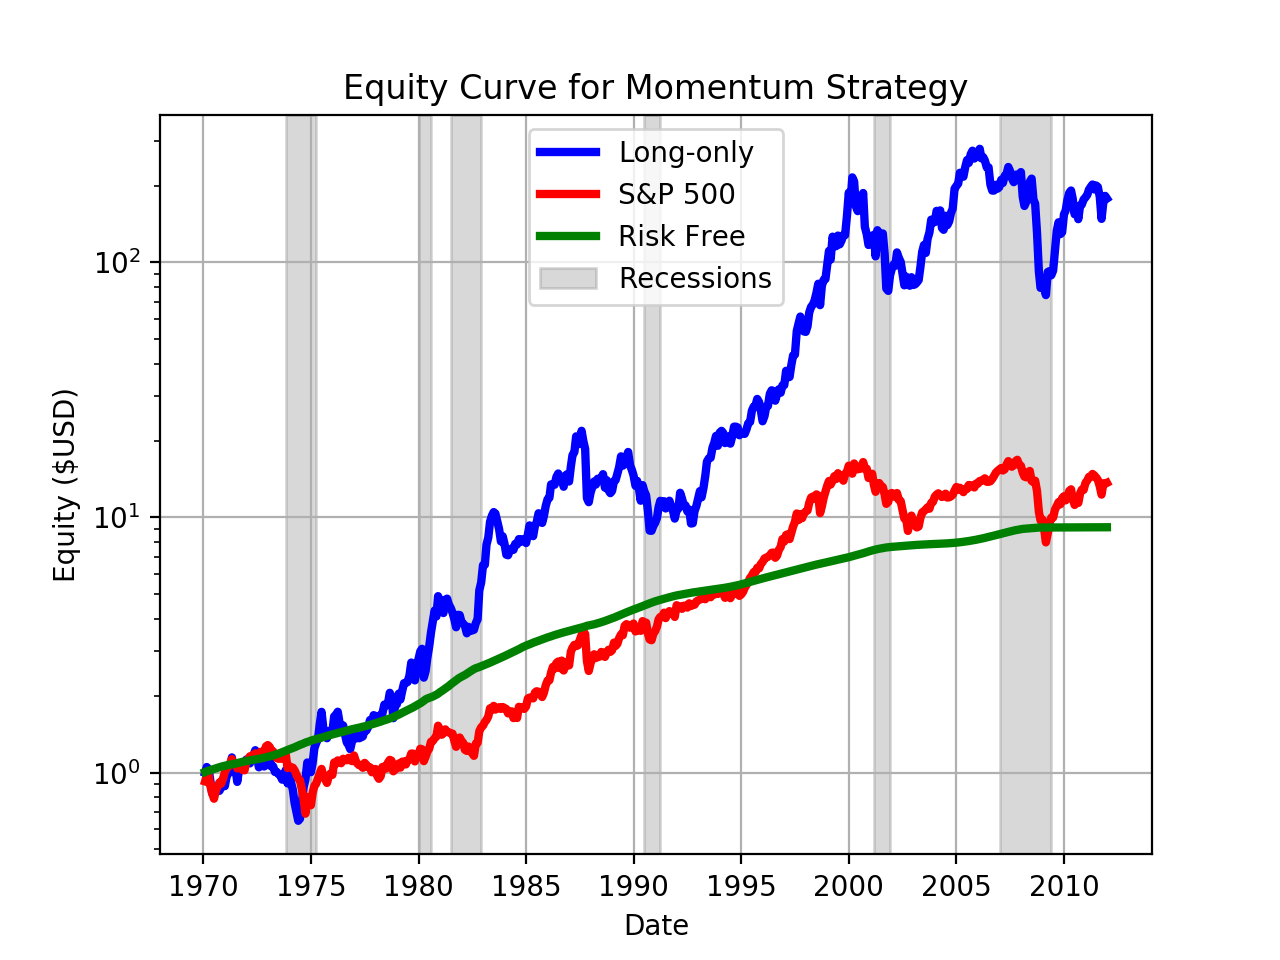
\includegraphics[width=\textwidth]{longonly.png} % first figure itself
        \caption{Long only momentum strategy}
        \label{fig:longonly}
    \end{minipage}\hfill
    \begin{minipage}{0.49\textwidth}
        \centering
        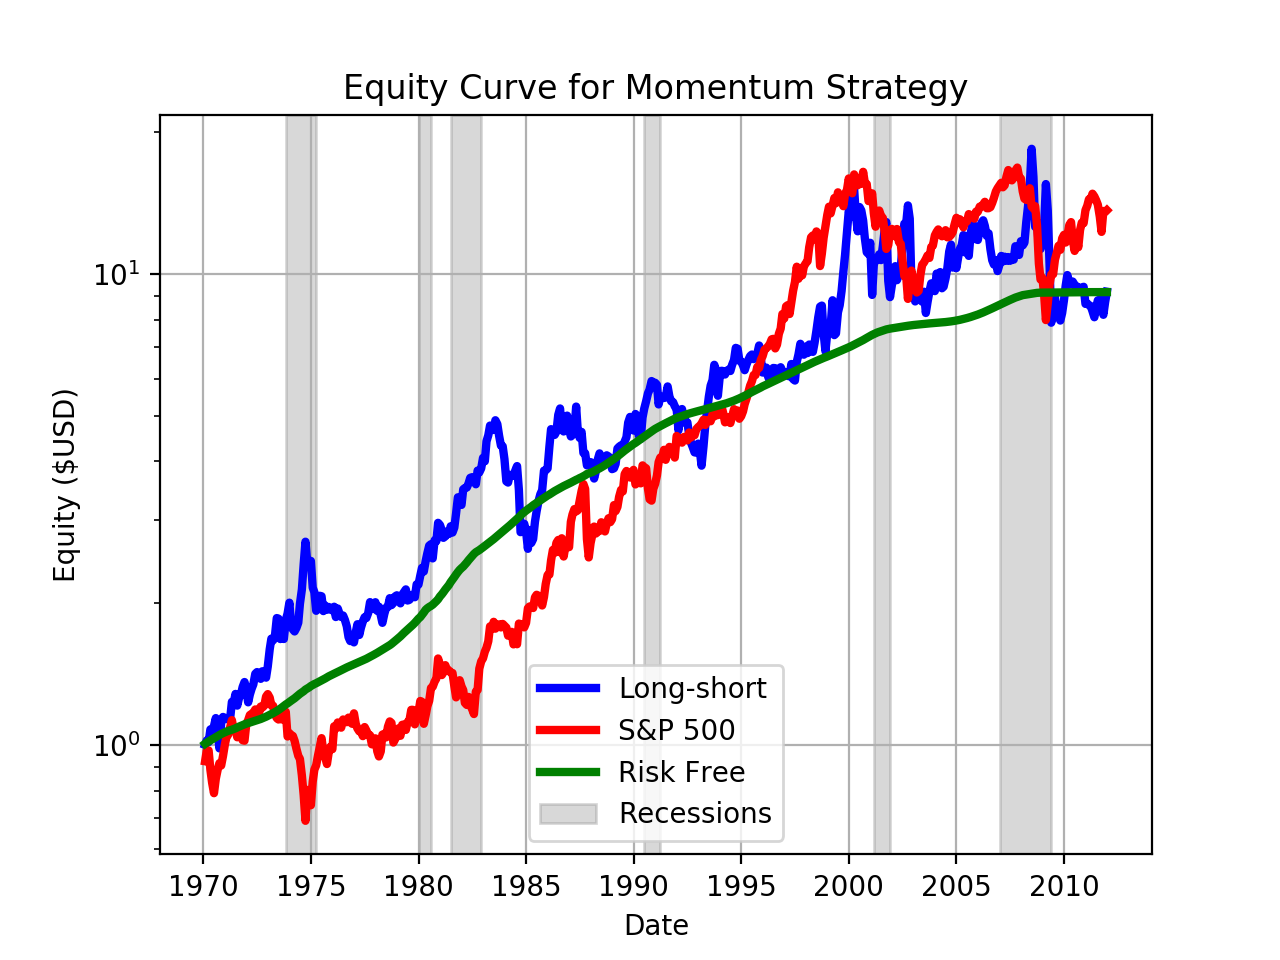
\includegraphics[width=\textwidth]{longshort.png} % second figure itself
        \caption{Long and short momentum strategy}
        \label{fig:longshort}
    \end{minipage}
\end{figure}


By looking at the long-only strategy we see that momentum indeed is vulnerable to crashes during periods of market decline (periods of recessions in the U.S. are highlighted in gray).  The largest dip occurs during the 2008 financial crisis.  We confirm in Figure~\ref{fig:timevarying} below that the three Fama-French factors are indeed dynamic with the momentum strategy exhibiting time-varying exposures with the exposures being the largest around the time of the 2008 recession. 

\begin{figure}[H]
\centering
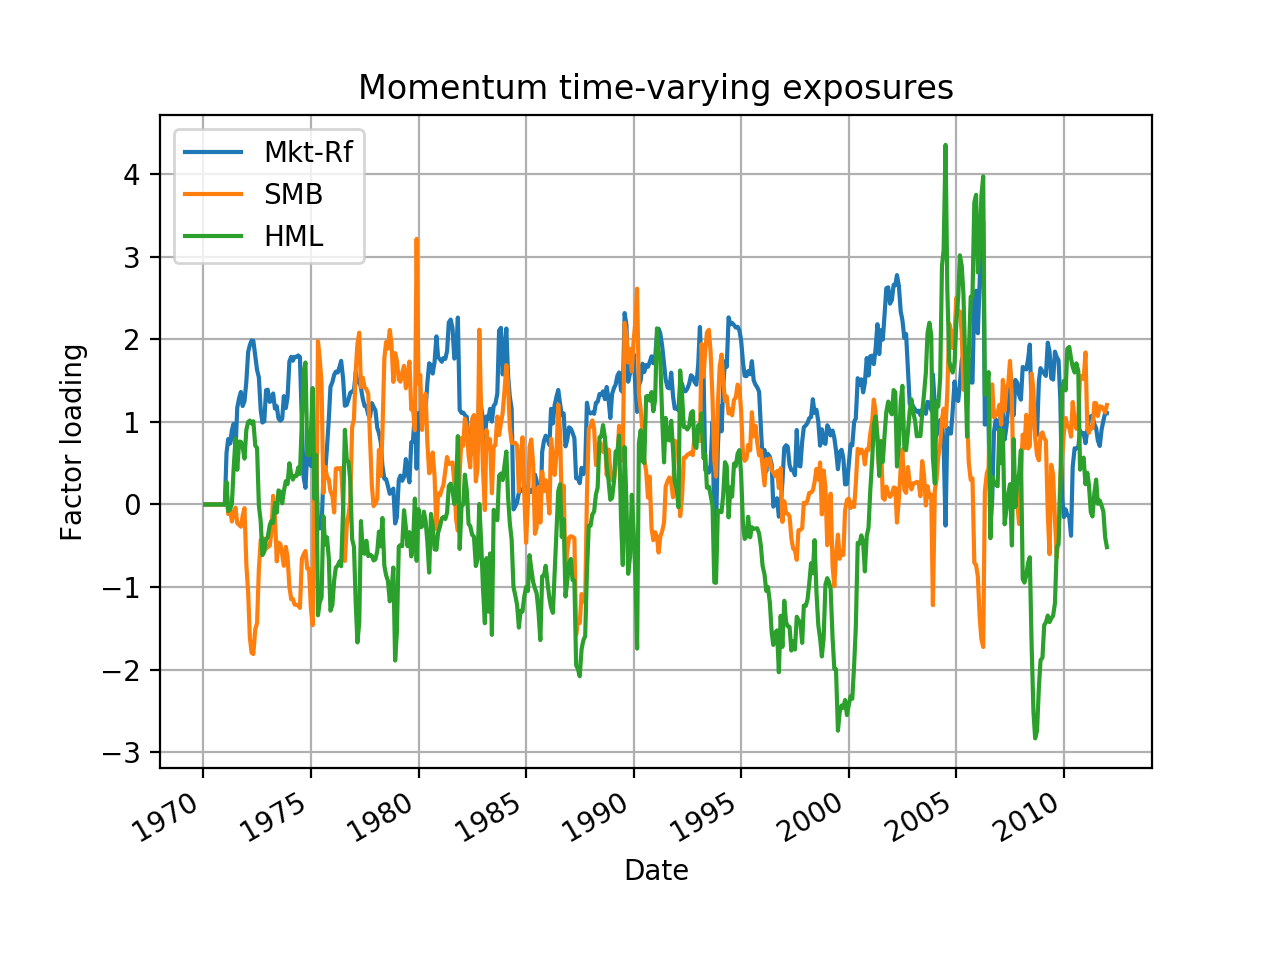
\includegraphics[width=\textwidth]{timevarying.png}
\caption{The three factor loadings $\tilde{\beta}_t, \tilde{s}_t, \tilde{h}_t$ for the long-only momentum strategy.  We use a 12 month rolling window for the regression.}
\label{fig:timevarying}
\end{figure}




\subsection{Main results}

In this section we compare the three momentum strategies to the benchmark S\&P 500 by backtesting from May 2012 to December 2019.  Note that data for the Invesco QQQ ETF was not available until May 2007 but, following Algorithm~\ref{algo:HMETF}, we need 5 months of previous data for the regression which is why the backtest starts on May 2012.  Figure~\ref{fig:comparison} shows the equity curves for these three strategies as well as the S\&P 500 benchmark and the risk-free returns given by the 1-month T-bill, while Table~\ref{table:summarystats} presents several summary statistics and performance metrics.\\

The first thing to note is that the factor loadings for the 3 Fama-French factors are reduced significantly for the the hedged strategies, particularly for the market risk and SMB factors.  This can also be seen with a lower max drawdown with the HMETF strategy have a smaller max drawdown than the S\&P 500.  However, this comes with the price of worse performance in terms of returns as the Sharpe and Sortino ratios are lower when compared to the unhedged strategy.  All three strategies perform better than the benchmark in almost all metrics measured.  While the hedged strategies are vastly outperformed by the unhedged strategy over this time period it is important to note two things: the first is that there were no recessions or market crashes during this period, which momentum is most vulnerable to, and second, that the hedged strategies indeed succeed in reducing their exposure.  From the second point one could conceivably leverage the hedged strategy to increase returns during uncertain times and market declines. \\

Interestingly enough, hedging with the ETFs reduces exposure to the Fama-French factors even more than hedging directly with the factors themselves.  This seems counter-intuitive and should be explored further, perhaps with different ETFs that have been around longer and thus have more data.  The factors, as well as the ETFs, are correlated and so theoretically one should take this into account when choosing the weights to hedge with.  Taking the covariance matrix into account one could derive better weights to improve performance.  We also note that other factor models include momentum as a factor, but here we would like to isolate the momentum anomaly and reduce our exposure to the other factors.  Ultimately this is just speculation without more data available.

\begin{table}[H]
\centering
\begin{tabular}{c | c | c | c | c}
Metric & Momentum (long-only) & HMFF3 & HMETF & S\&P 500 \\
\hline
Average Return \% & 2.483 & 1.028 &  0.570 & 0.965 \\
Standard Deviation \% & 5.294 & 2.347 & 4.250 & 3.172 \\
Alpha & 0.014 & 0.006 & 0.006 & -0.002 \\
Beta & 0.992 & 0.412 & 0.256 & 0.980 \\
SMB & 0.253 & 0.091 & 0.014 & -0.136 \\
HML & 0.039 & 0.083 & 0.034 & -0.014 \\
$R^2$ & 0.434 &  0.382 & 0.159 & 0.995\\
Sharpe & 1.578 & 1.425 & 1.379 & 0.991  \\
Sortino & 4.032 & 3.846 & 3.568 &  1.705 \\
Max Drawdown & 0.882 & 0.600 & 0.563 & 0.594
\end{tabular}
\caption{Backtest summary statistics for the three momentum strategies as well as the S\&P 500 benchmark.  The average returns and standard deviations are monthly whereas the Sharpe and Sortino ratios are annualized.  Note that for the three momentum strategies transaction costs of 5 basis points each way (buying and selling) were added.}
\label{table:summarystats}
\end{table}


\begin{figure}[H]
\centering
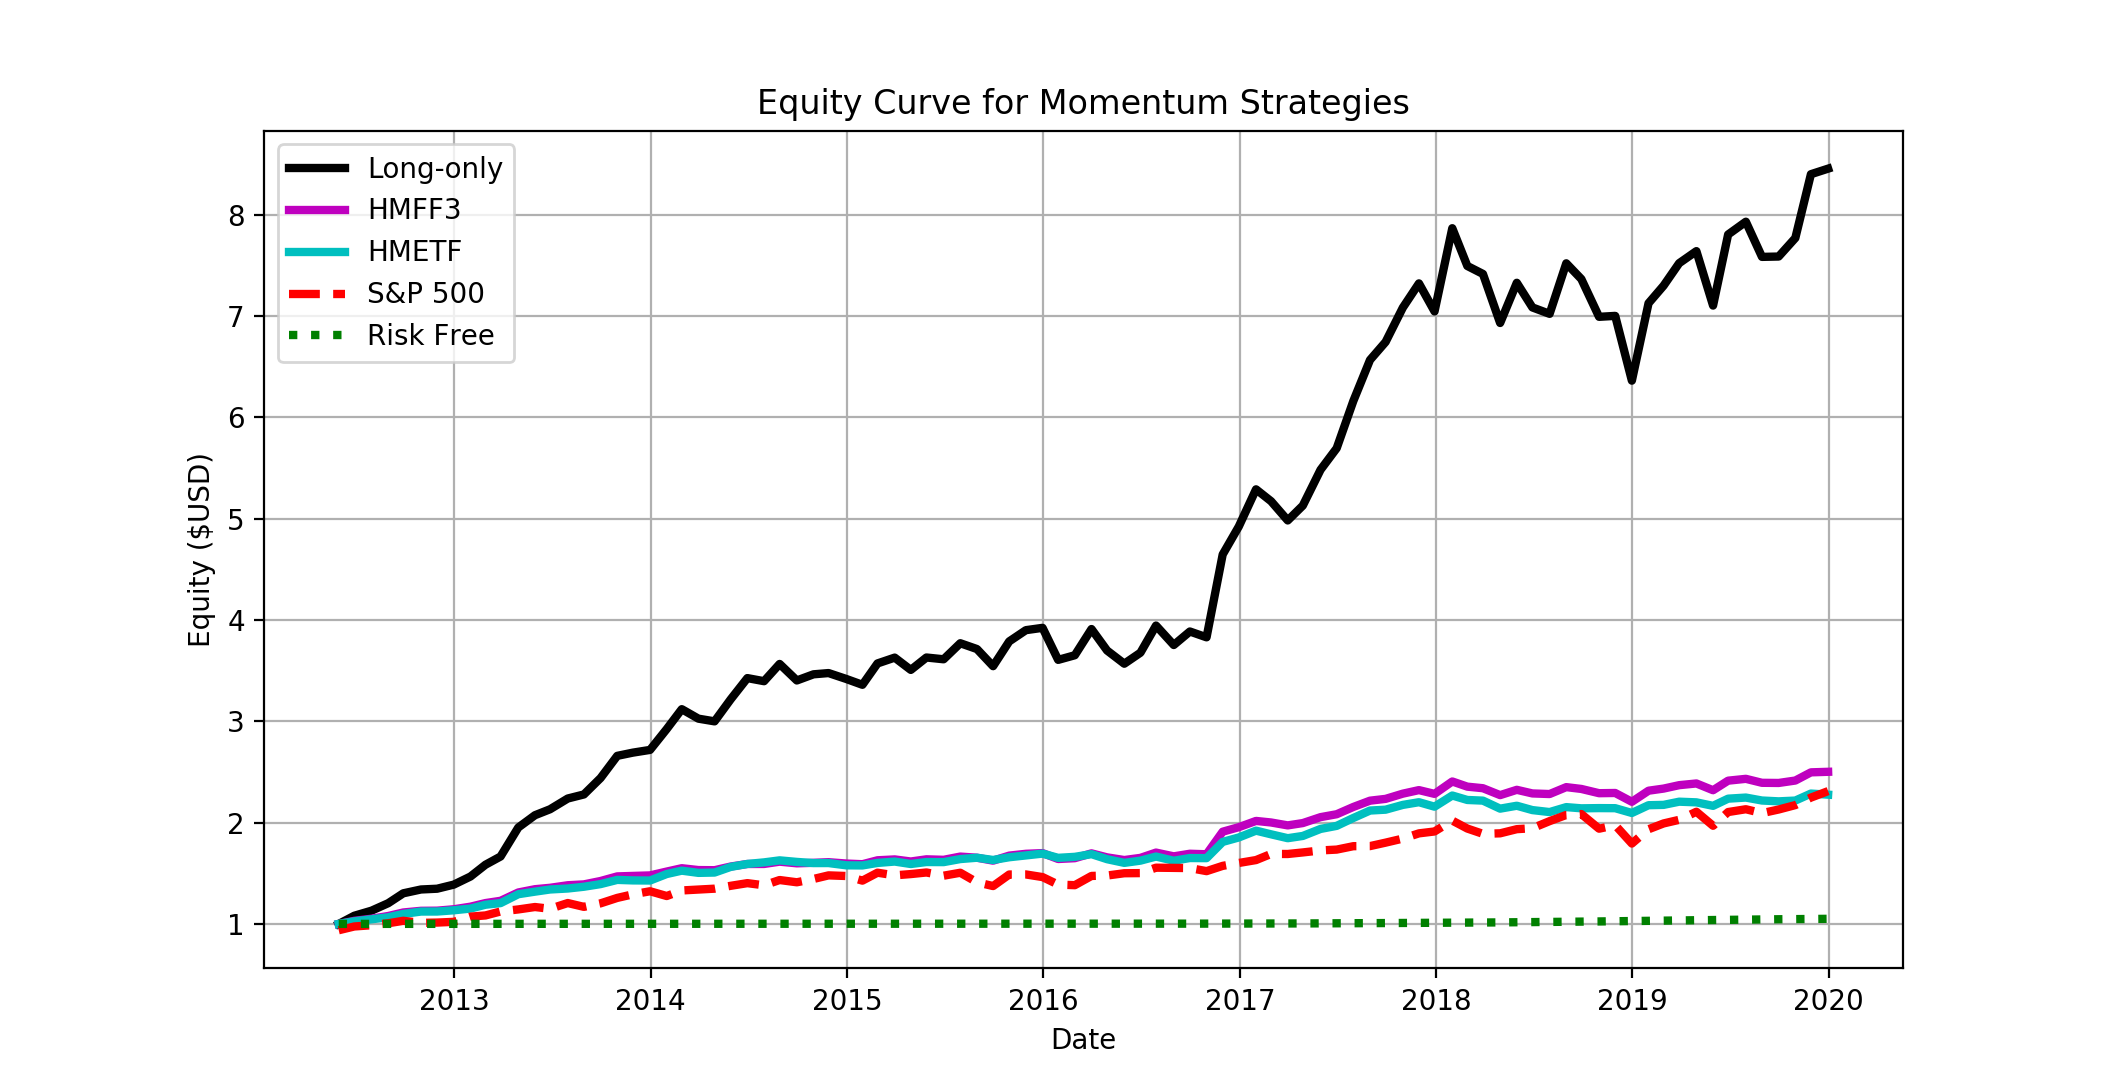
\includegraphics[width=\textwidth]{comparison.png}
\caption{}
\label{fig:comparison}
\end{figure}



\subsection{Transaction costs}

For all of the backtests above we have assumed a fixed rate of 5 basis points (bp) for the transaction costs (x-costs) both ways.  However, a better model might have separate transaction costs for the equities and the ETFs.  Indeed some actively managed ETFs also have separate fees.  Instead we focus on the compounding effect of increasing the transaction cost by backtesting the long-only and unhedged momentum strategy from January 1970 to December 2019.  Figure~\ref{fig:xcost_comparison} shows the results for fixed transaction costs of 0, 5, 15, and 50 basis points.  As expected, we see that increasing the transaction costs decreases the profitability of the strategy.  However, even with very steep costs of 50 basis points each direction we still find that the long-only momentum strategy consistently outperforms the S\&P 500 benchmark.  Over a long period of time, the strategy performs very well and with small transaction costs one could have made around 100 times as much money when compared to investing in the risk-free asset only.  Of course, this is over a period of nearly 50 years.  The modest rate of 5 basis points is somewhat reasonable because we only trade typically large-cap stocks that are on the S\&P 500 so we do not need to worry too much about smaller-cap stocks that are less liquid and carry higher fees.

\begin{figure}[H]
\centering
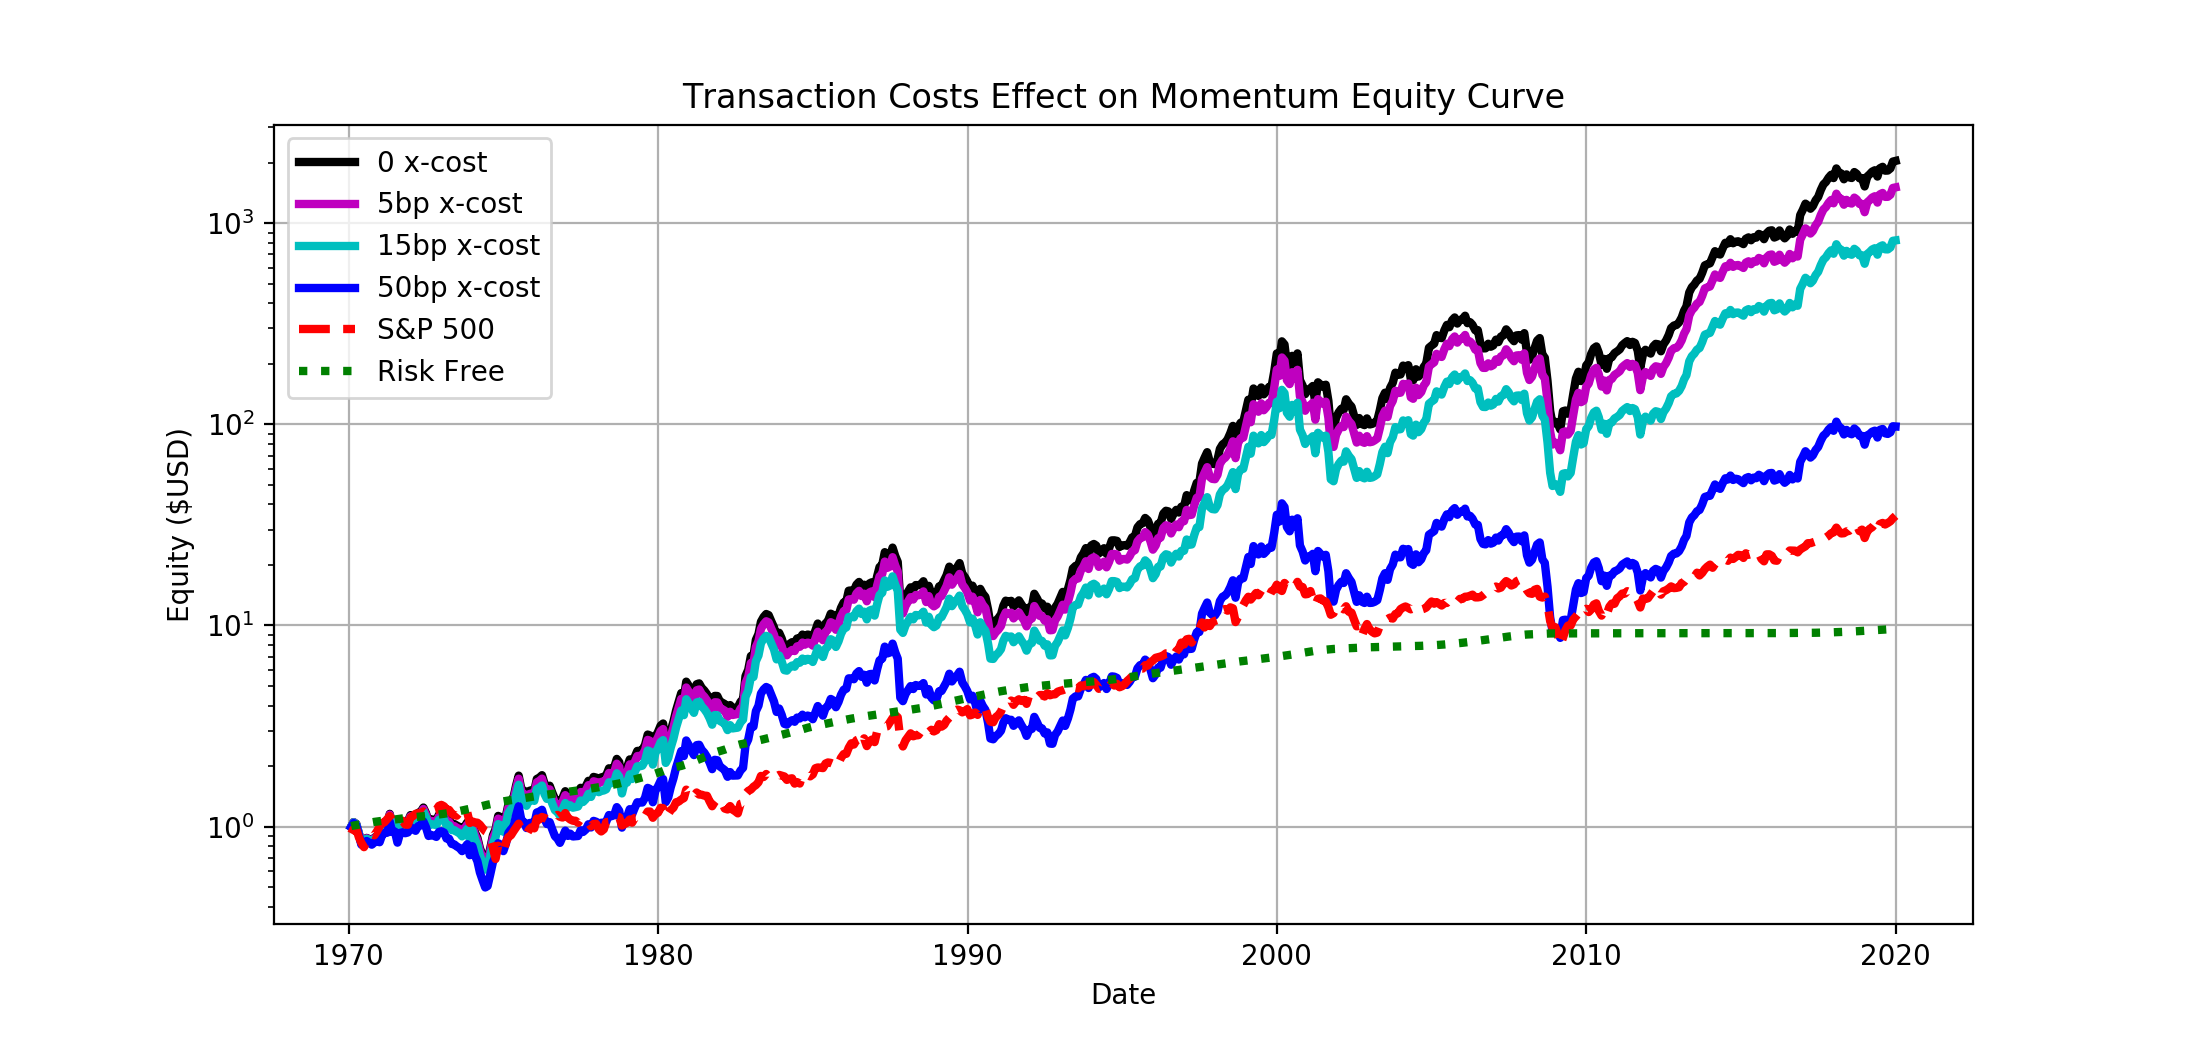
\includegraphics[width=\textwidth]{xcost_comparison.png}
\caption{The performance of the long-only momentum strategy with different transaction costs from 1970 to 2019.}
\label{fig:xcost_comparison}
\end{figure}



\section{Conclusions and outlook}

We have already noted some areas for future improvement.  First one could consider using different ETFs or even allow the strategy to change ETFs over time.  To do this one would need to select a criteria for which ETFs are good to hedge with.  One idea could be to choose ETFs that closely follow the sectors of the stocks that are picked.  For example, if the top 5 returning stocks from the 6 month lookback period are all tech stocks, one may wish to use a tech ETF to hedge with.  Another criteria could be simply to find which ETFs replicate the Fama-French factors, or some other factor model, as closely as possible.  This approach is more in line with what I have done in this report.\\

Another direction for future research would be to look at different time periods.  While these algorithms perform well from 2012 up until 2019, we do not know how they would perform more recently with the COVID crisis where there was a steep drop in stock prices and then a swift rebound.  One could perhaps get an idea by studying the performance of the strategy during a different historical period containing a recession or other market crash.  However, one has to balance the lookback period (number of observations for the regression) and which ETFs are available.  For instance, the QQQ ETF is still fairly recent.  This goes back to the first point of choosing different ETFs.\\

Momentum strategies have been shown to be effective historically as well as currently, but are susceptible to crashes.  These crashes can be hedged against by reducing exposure to the Fama-French factors.  The work \cite{MvO} have attempted this with the Fama-French factors.  However, this is not practical and so I propose to use ETFs that approximate the factors instead.  I find that hedging this way indeed reduces the exposure to the factors significantly, but comes at the cost of worse performance than the unhedged strategy.  It would be interesting to see how this approach performs during a market decline as well as to try one of the different hedging strategies proposed in \cite{MvO}.


\nocite{*}
\bibliographystyle{unsrt}
\bibliography{references}



\end{document}